\section{Neutron Diffusion Results}
\label{sec:diffusionResults}

\begin{frame}{Verification and Validation}
  \begin{itemize}
    \item Comparison against analytic solutions and benchmark problems.
    \item Strategy from \cite{oberkampf}.
    \item ``Code Verification''
      \begin{itemize}
        \item Compare computational results to exact analytic or manufactured
          results.
        \item Demonstrate the code is solving equations correctly as designed.
        \item Quantified numerical errors.
      \end{itemize}
    \item ``Solution Verification''
      \begin{itemize}
        \item Compare computational results to benchmark results for the
          intended application of the solver.
        \item Computational results from a different method or experimental
          data.
        \item Typically verified by others previously.
      \end{itemize}
  \end{itemize}
\end{frame}

\begin{frame}{Error Analysis}
  FEM with linear elements is second-order convergent in space
  \cite{textbookli}.
  \begin{equation} 
    \label{eq:error_bound}
    \|\ve\|_{\infty} \le c h^2 \| \grad^2 \phi(\vr) \|_{\infty}
  \end{equation}
  It is useful to define the following errors.
  \begin{align}
    \ve &= \phi(\vr) - \phi_{FEM} \\
    \label{eq:rms}
    \text{RMS}(\ve) &= \sqrt{\frac{1}{N} \sum_{i=1}^{N} e_i^2} \\
    \label{eq:infnorm}
    \|\ve\|_{\infty} &= \max_{i=1,2,\ldots,N} \lvert e_i \rvert
  \end{align}
\end{frame}

\begin{frame}{One-Dimension, One-Group, Fixed Source}
  \begin{table}
    %\caption{One-Dimension, One-Group, Fixed Source Convergence Study 
    %  Results.}
    \label{tab:1dfixedsrc}
    \begin{center}
      \begin{tabular}{ccccc}
        \toprule
        Refine & RMS & RMS ratio & $\|e\|_{\infty}$ & 
          $\|e\|_{\infty}$ ratio \\
        \midrule
        \csvreader[
          late after line=\\,
          late after last line=\\\bottomrule,]
          {../ch03_diffusionResults/data/1dfixedsrc.csv}{}
          {\csvcoli & \csvcolii & \csvcoliii & \csvcolviii & \csvcolix}
      \end{tabular}
    \end{center}
  \end{table}
  \begin{equation}
    \label{eq:analytic_1dfixedsrc}
    \phi(x) = \left( \frac{q_{fixed}}{D} \right) 
      \left( 1-\cosh(\kappa\,x) +
      \frac{\cosh(\kappa\,L_x)-1}{\sinh(\kappa\,L_x)}
      \sinh(\kappa\,x)\right)
  \end{equation}
\end{frame}

\begin{frame}{One-Dimension, One-Group, Criticality}
  \begin{table}
    %\caption{One-Dimension, One-Group, Criticality Convergence Study
    %  Results.}
    \label{tab:1d1g}
    \begin{center}
      \resizebox{\textwidth}{!}{
      \begin{tabular}{cccccccccc}
        \toprule
        Refine & $\keff$ & $\keff$ error \units{pcm} & $\keff$ ratio & RMS & 
          RMS ratio  & $\|e\|_{\infty}$ & $\|e\|_{\infty}$ ratio \\
        \midrule
        \csvreader[
          late after line=\\,
          late after last line=\\,]
          {../ch03_diffusionResults/data/1d1g.csv}{}
          {\csvcoli & \csvcolii & \csvcoliii & \csvcoliv & \csvcolv & 
          \csvcolvi & \csvcolxi & \csvcolxii}
        Ref. & 1.998028 \\
        \bottomrule
      \end{tabular}
    }
    \end{center}
  \end{table}
  \begin{equation}
    \label{eq:analytic_1d1g}
    \phi(x) = \phi_0 \, \sin\left(\frac{\pi}{L_x} x \right)
  \end{equation}
\end{frame}

\begin{frame}{One-Dimension, One-Group Plots}
  \begin{figure}
    \centering
    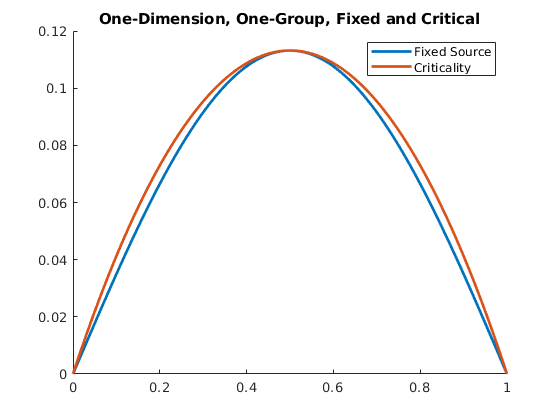
\includegraphics[width=0.7\textwidth]{fixed_critical}
    \caption{Fixed Source and Criticality Flux Shapes for One-Dimension,
      One-Group Problems.}
    \label{fig:fixed_critical}
  \end{figure}
\end{frame}

\begin{frame}{Two-Dimension, One-Group, Criticality}
  \begin{table}
    %\caption{Two-Dimension, One-Group, Criticality Convergence Study
    %  Results.}
    \label{tab:2d1g}
    \begin{center}
      \resizebox{\textwidth}{!}{
      \begin{tabular}{cccccccccc}
        \toprule
        Refine & $\keff$ & $\keff$ error \units{pcm} & $\keff$ ratio & RMS & 
          RMS ratio  & $\|e\|_{\infty}$ & $\|e\|_{\infty}$ ratio \\
        \midrule
        \csvreader[
          late after line=\\,
          late after last line=\\,]
          {../ch03_diffusionResults/data/2d1g.csv}{}
          {\csvcoli & \csvcolii & \csvcoliii & \csvcoliv & \csvcolv & 
          \csvcolvi & \csvcolxi & \csvcolxii}
        Ref. & 1.996060  \\
        \bottomrule
      \end{tabular}
    }
    \end{center}
  \end{table}
  \begin{equation}
    \label{eq:analytic_2d1g}
    \phi(x,y) = \phi_0 \sin\left(\frac{\pi}{L_x} x\right) \, 
      \sin\left(\frac{\pi}{L_y} y\right)
  \end{equation}
\end{frame}

\begin{frame}{Two-Dimension, One-Group, Criticality}
  \begin{figure}
    \centering
    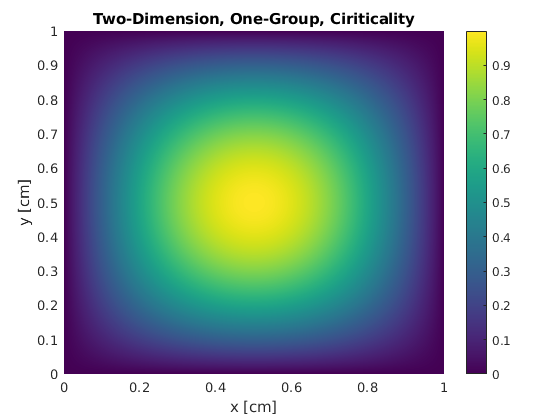
\includegraphics[width=0.7\textwidth]{2d1g}
    \caption{Two-Dimension Criticality Flux Shape.}
    \label{fig:2d1g}
  \end{figure}
\end{frame}

\begin{frame}{One-Dimension, Two-Group, Criticality}
  \begin{table}
    %\caption{One-Dimension, Two-Group, Criticality Convergence Study
    %  Results.}
    \label{tab:1d2g}
    \begin{center}
      \resizebox{\textwidth}{!}{
      \begin{tabular}{ccccccc}
        \toprule
        Refine & $\keff$ & $\keff$ error \units{pcm} & $\keff$ ratio & 
          $\phi_2/\phi_1$ & $\phi_2/\phi_1$ error & $\phi_2/\phi_1$ ratio \\
        \midrule
        \csvreader[
          late after line=\\,
          late after last line=\\,]
          {../ch03_diffusionResults/data/1d2g.csv}{}
          {\csvcoli & \csvcolii & \csvcoliii & \csvcoliv & \csvcolv & 
          \csvcolvi & \csvcolvii}
        Ref. & 0.892349 &  &  & 0.261324 \\
        \bottomrule
      \end{tabular}
    }
    \end{center}
  \end{table}
  \begin{align}
    \phi_1(x) &= \phi_0 \, \sin\left(\frac{\pi}{L_x} x \right), \\
    \phi_2(x) &= \frac{k_2}{k_1} \, \phi_0 \, \sin\left(\frac{\pi}{L_x} x
      \right), \\
    \frac{k_2}{k_1} &= \frac{\Sigma_{s 1\rightarrow 2}}{D_2 \,
      \left(\frac{\pi}{L_x}\right)^2 + \Sigma_{r2}}
  \end{align}
\end{frame}

\begin{frame}{One-Dimension, Two-Group, Criticality}
  \begin{figure}
    \centering
    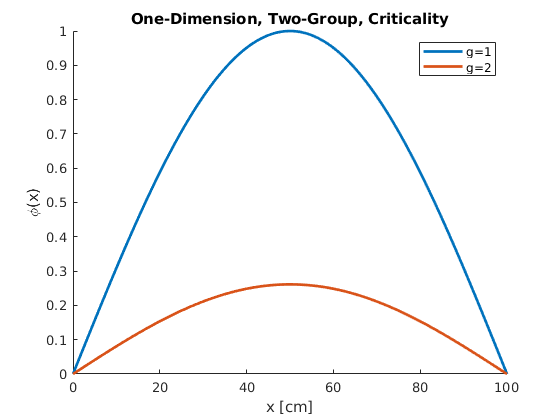
\includegraphics[width=0.7\textwidth]{1d2g}
    \caption{Example Two-Group Flux Plot.}
    \label{fig:1d2g}
  \end{figure}
\end{frame}

\begin{frame}{One-Dimension, One-Group, Two Region, Criticality}
  \begin{table}
    %\caption{One-Dimension, One-Group, Two-Region, Criticality Convergence
    %  Study Results.}
    \label{tab:2reg}
    \begin{center}
      \resizebox{\textwidth}{!}{
      \begin{tabular}{cccccccccc}
        \toprule
        Refine & $\keff$ & $\keff$ error \units{pcm} & $\keff$ ratio & RMS & 
          RMS ratio  & $\|e\|_{\infty}$ & $\|e\|_{\infty}$ ratio \\
        \midrule
        \csvreader[
          late after line=\\,
          late after last line=\\,]
          {../ch03_diffusionResults/data/2reg.csv}{}
          {\csvcoli & \csvcolii & \csvcoliii & \csvcoliv & \csvcolv & 
          \csvcolvi & \csvcolxi & \csvcolxii}
        Ref. & 0.962188 \\
        \bottomrule
      \end{tabular}
    }
    \end{center}
  \end{table}
  \begin{align}
    \phi_F(x) &= \phi_0 \, \cos(B_F \, x) \\
    \phi_R(x) &= \phi_0 \, \cos(B_F \, L_F) \, \cosh(\kappa_R \, (x-L_F)) - 
      \frac{\phi_0 \, D_F \, B_F \, \sin(B_F\,L_F)}{D_R \, \kappa_R} \, 
      \sinh(\kappa_R\,(x-L_F)) \\
    \label{eq:analytic_2reg}
    %\phi(x) &= H(x-L_F) \, \phi_R(x) + H(L_F-x) \, \phi_F(x)
    \phi(x) &=
    \begin{cases}
      \phi_F(x) & 0   \le x \le L_F \\
      \phi_R(x) & L_F \le x \le L_R
    \end{cases}
  \end{align}
\end{frame}

\begin{frame}{One-Dimension, One-Group, Two Region, Criticality}
  \begin{figure}
    \centering
    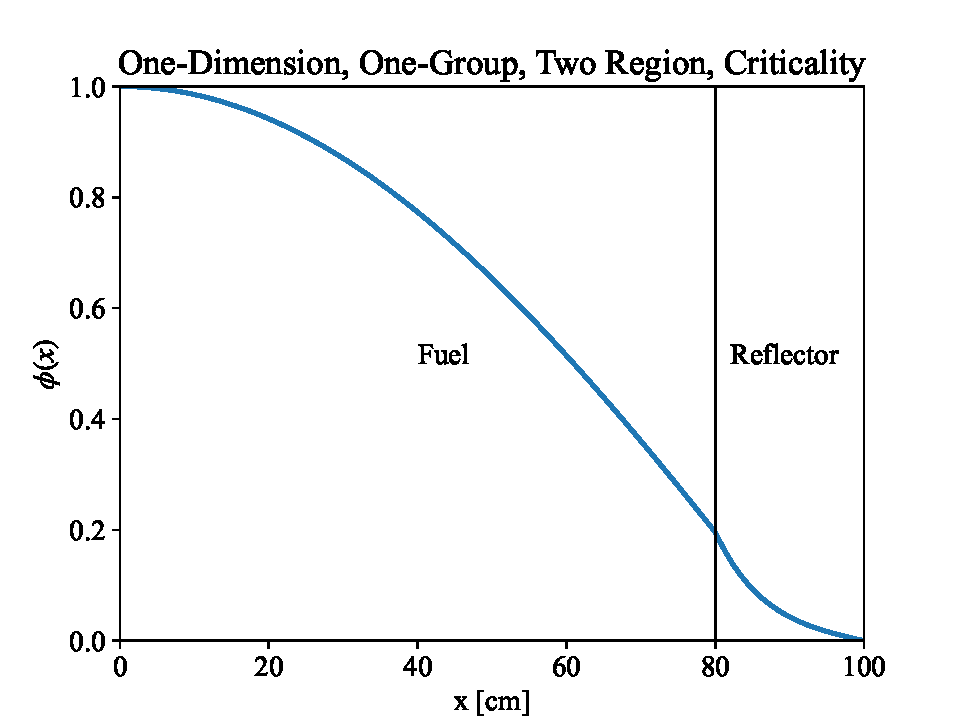
\includegraphics[width=0.7\textwidth]{2reg}
    \caption{Two Region Flux Shape.}
    \label{fig:2reg}
  \end{figure}
\end{frame}

\begin{frame}{Three-Dimension, One-Group, Finite Cylinder}
  \begin{table}
    %\caption{Finite Cylinder Convergence Study Results.}
    \label{tab:finite_cyl}
    \begin{center}
      \resizebox{\textwidth}{!}{
      \begin{tabular}{cccccccccc}
        \toprule
        Refine & $\keff$ & $\keff$ error \units{pcm} & $\keff$ ratio & RMS & 
          RMS ratio  & $\|e\|_{\infty}$ & $\|e\|_{\infty}$ ratio \\
        \midrule
        \csvreader[
          late after line=\\,
          late after last line=\\,]
          {../ch03_diffusionResults/data/finite_cyl.csv}{}
          {\csvcoli & \csvcolii & \csvcoliii & \csvcoliv & \csvcolv & 
          \csvcolvi & \csvcolxi & \csvcolxii}
        Ref. & 0.996711 \\
        \bottomrule
      \end{tabular}
    }
    \end{center}
  \end{table}
  \begin{equation}
    \label{eq:analytic_finite_cyl}
    \phi(r,z) = \phi_0 \, 
      J_0\left(\frac{\alpha_0}{T} r\right) \sin\left(\frac{\pi}{H} z \right)
  \end{equation}
\end{frame}

\begin{frame}{Three-Dimension, One-Group, Finite Cylinder}
  \begin{figure}
    \centering
    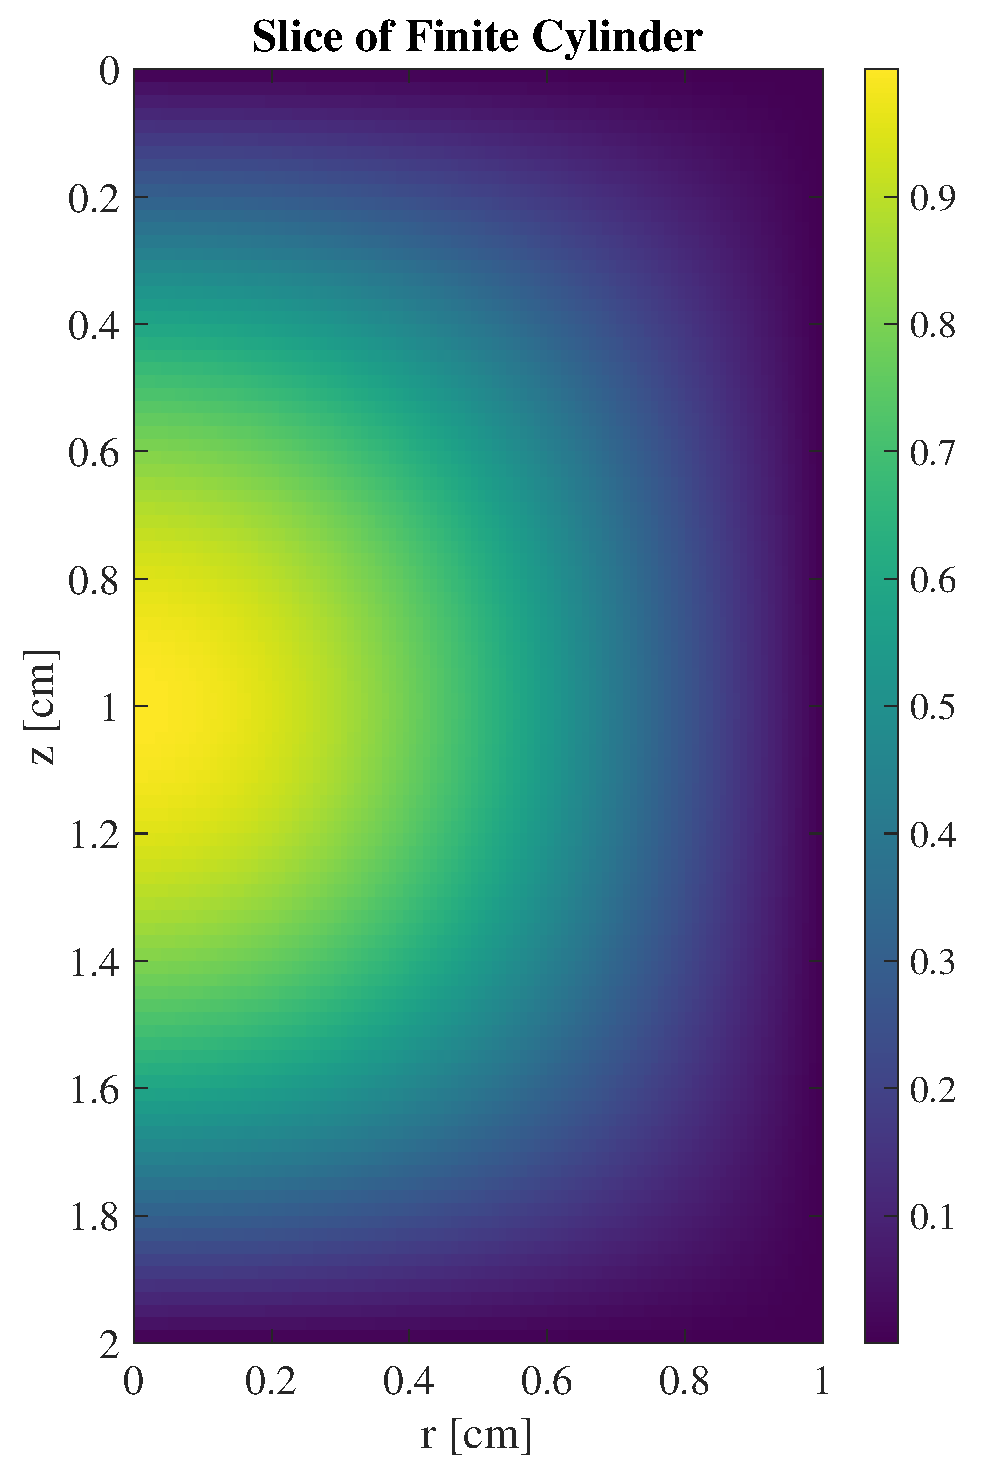
\includegraphics[width=0.4\textwidth]{finite_cyl}
    \caption{Example Finite Cylinder Flux Shape.}
    \label{fig:finite_cyl}
  \end{figure}
\end{frame}

\begin{frame}{VVER440}
  \begin{itemize}
    \item Two-dimensional.
    \item Light Water Reacotr (LWR).
    \item Two-group.
  \end{itemize}
  \begin{table}
    \begin{center}
      %\caption{VVER440 Benchmark Convergence Study.}
      \label{tab:vver440}
      \begin{threeparttable}
        \begin{tabular}{cccc}
          \toprule
          Refine & $\keff$ & $\keff$ error \units{pcm} & $\keff$ ratio \\
          \midrule
          \csvreader[
            late after line=\\,
            late after last line=\\,]
            {../ch03_diffusionResults/data/vver440.csv}{}
            {\csvcoli & \csvcolvi & \csvcolvii & \csvcolviii}
          Ref.\tnote{$\dagger$}  & 1.009700 \\
          \bottomrule
        \end{tabular}
        \begin{tablenotes}
          \item[$\dagger$] See \cite{chao}.
        \end{tablenotes}
      \end{threeparttable}
    \end{center}
  \end{table}
\end{frame}

\begin{frame}{VVER440 Benchmark Power Comparison}
  \begin{figure}
    \centering
    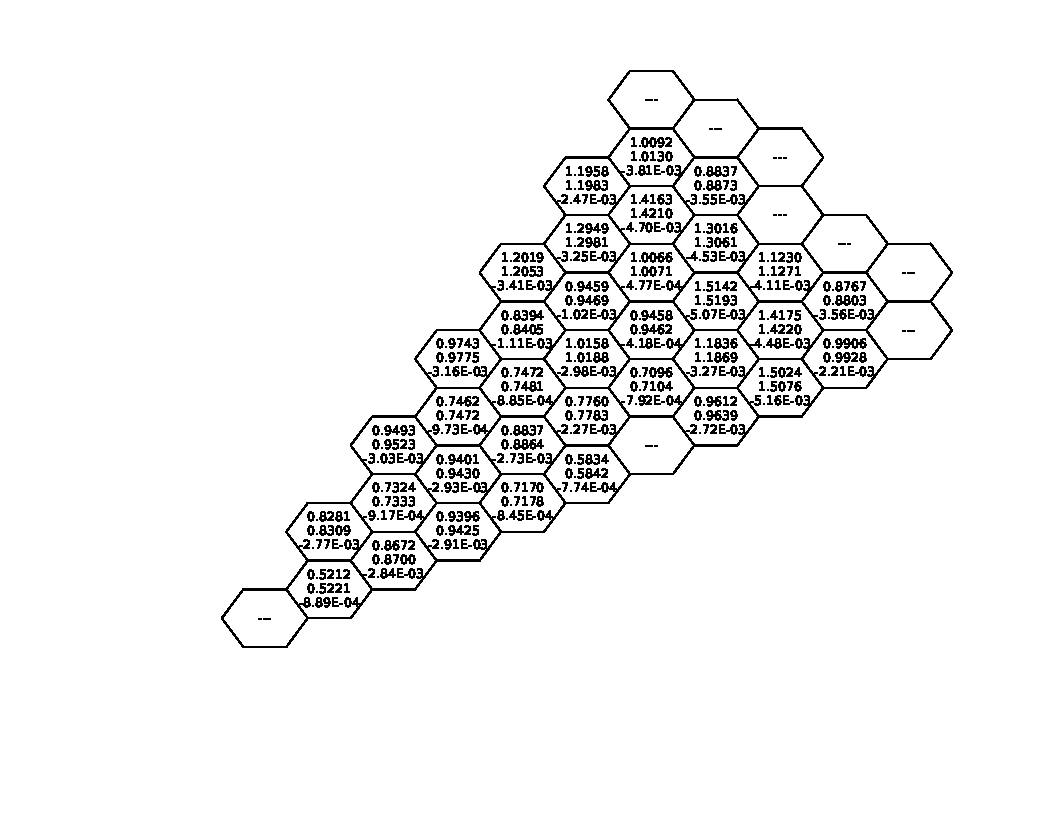
\includegraphics[width=\textwidth]{diffusion_vver440}
    %\caption{VVER440 Benchmark Power Comparison for Most Refined Mesh.}
    \label{fig:diffusion_vver440}
  \end{figure}
  \Put(25,450){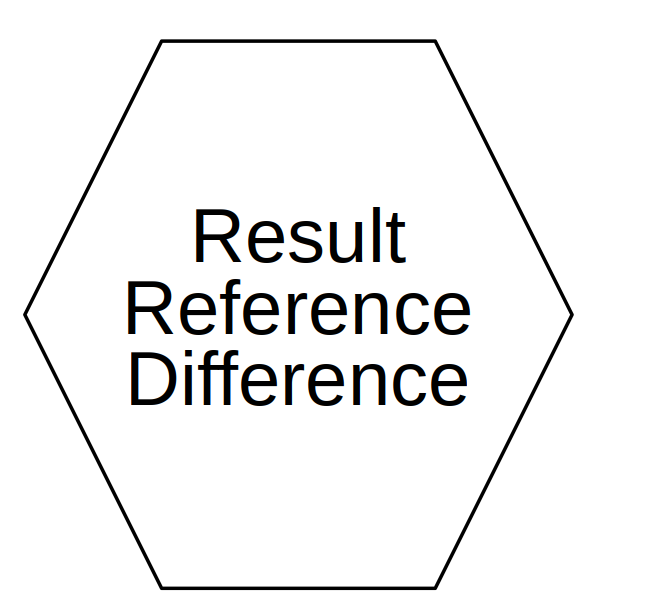
\includegraphics[width=0.15\textwidth]{hex_description}}
\end{frame}

\begin{frame}{SNR}
  \begin{itemize}
    \item Two-dimensional.
    \item Sodium-cooled Fast Reactor (SFR).
    \item Four-group.
  \end{itemize}
  \begin{table}
    \begin{center}
      %\caption{SNR Benchmark Convergence Study.}
      \label{tab:snr}
      \begin{threeparttable}
        \begin{tabular}{cccc}
          \toprule
          Refine & $\keff$ & $\keff$ error \units{pcm} & $\keff$ ratio \\
          \midrule
          \csvreader[
            late after line=\\,
            late after last line=\\,]
            {../ch03_diffusionResults/data/snr.csv}{}
            {\csvcoli & \csvcolvi & \csvcolvii & \csvcolviii}
          Ref. \tnote{$\dagger$} & 1.124000 \\
          \bottomrule
        \end{tabular}
        \begin{tablenotes}
          \item[$\dagger$] See \cite{argonneBenchmark}.
        \end{tablenotes}
      \end{threeparttable}
    \end{center}
  \end{table}
\end{frame}

\begin{frame}{SNR Benchmark Power Comparison}
  \begin{figure}
    \centering
    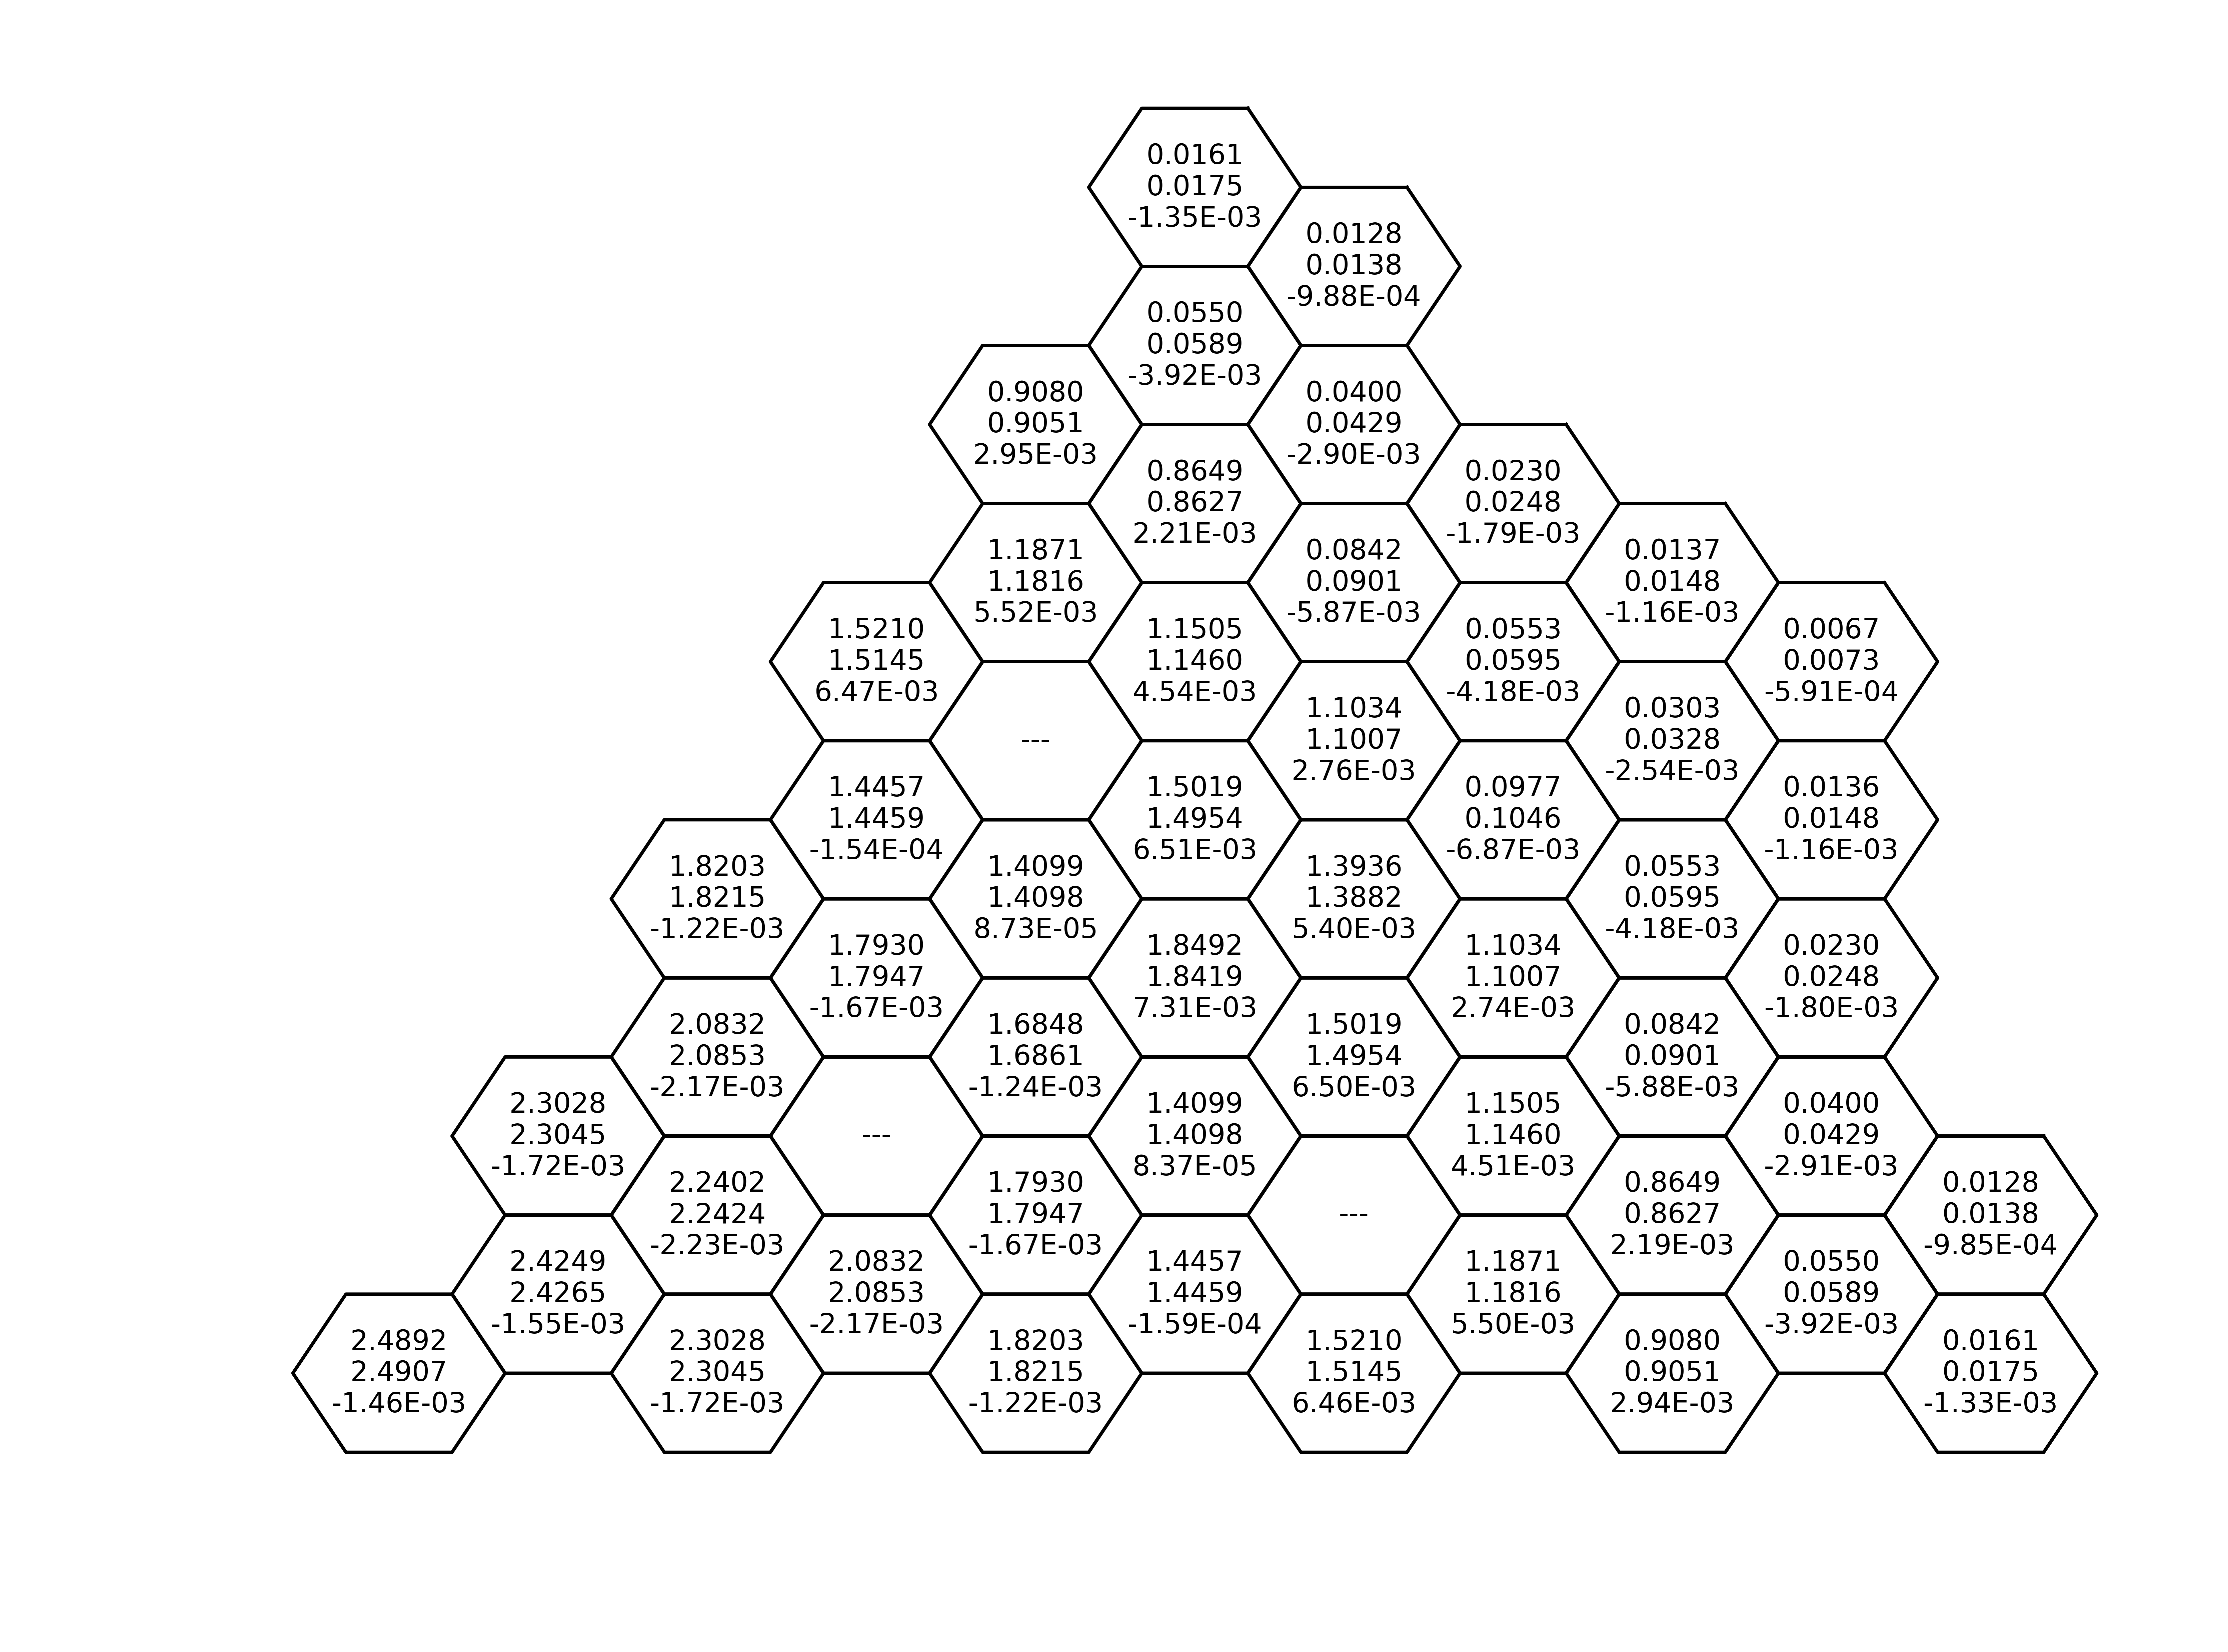
\includegraphics[width=\textwidth]{diffusion_snr}
    %\caption{SNR Benchmark Power Comparison for Most Refined Mesh.}
    \label{fig:diffusion_snr}
  \end{figure}
  \Put(25,450){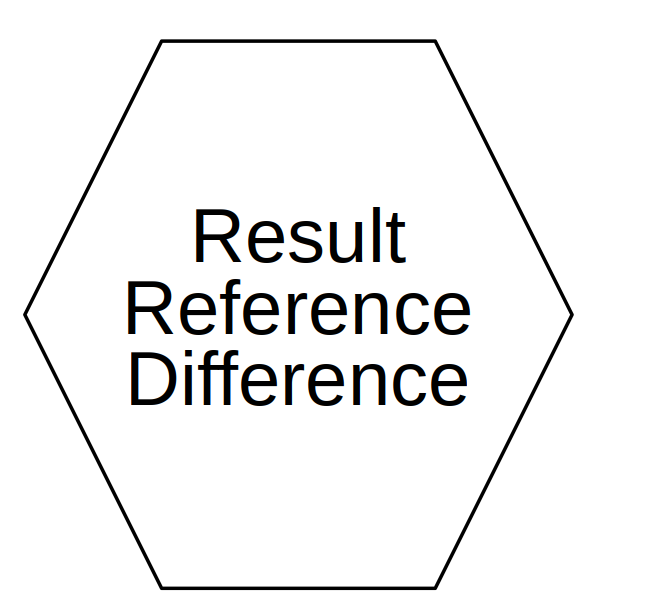
\includegraphics[width=0.15\textwidth]{hex_description}}
\end{frame}

\begin{frame}{HWR}
  \begin{itemize}
    \item Two-dimensional.
    \item Heavy Water Reactor (HWR).
    \item Two-group.
  \end{itemize}
  \begin{table}
    \begin{center}
      %\caption{HWR Benchmark Convergence Study.}
      \label{tab:hwr}
      \begin{threeparttable}
        \begin{tabular}{cccc}
          \toprule
          Refine & $\keff$ & $\keff$ error \units{pcm} & $\keff$ ratio \\
          \midrule
          \csvreader[
            late after line=\\,
            late after last line=\\,]
            {../ch03_diffusionResults/data/hwr.csv}{}
            {\csvcoli & \csvcolvi & \csvcolvii & \csvcolviii}
          Ref.\tnote{$\dagger$} & 0.991965  \\
          \bottomrule
        \end{tabular}
        \begin{tablenotes}
          \item[$\dagger$] See \cite{chao}.
        \end{tablenotes}
      \end{threeparttable}
    \end{center}
  \end{table}
\end{frame}

\begin{frame}{HWR Benchmark Power Comparison}
  \begin{figure}
    \centering
    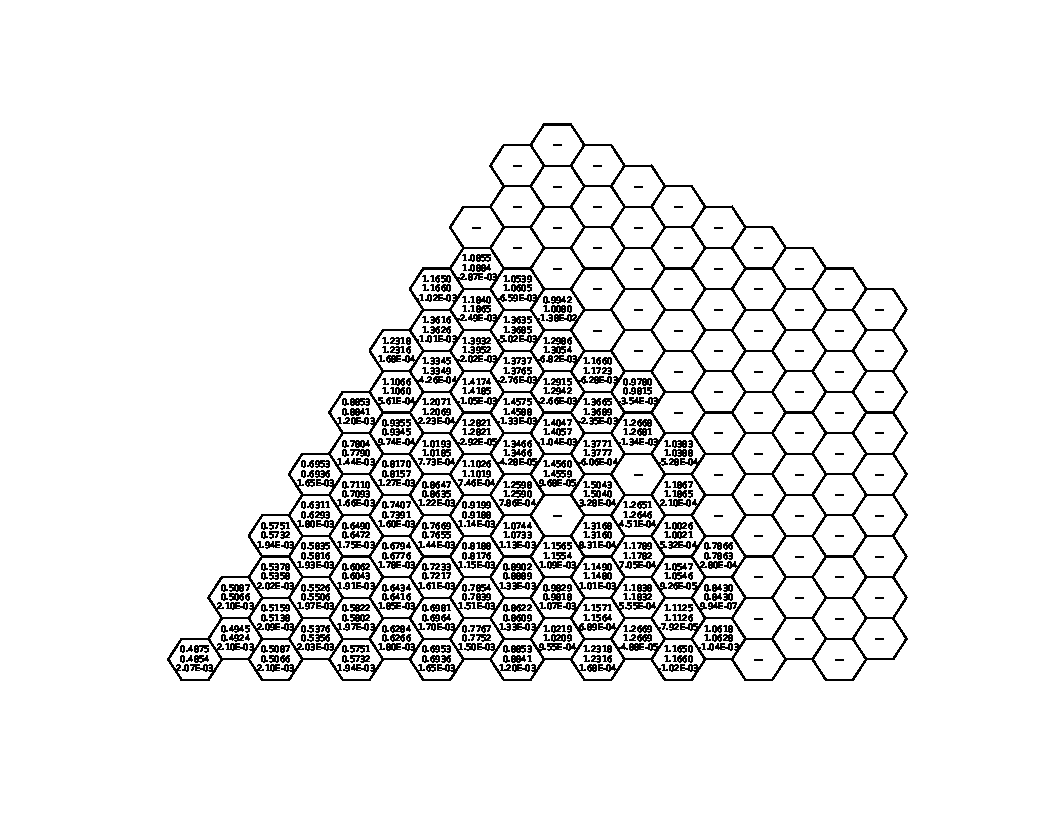
\includegraphics[width=\textwidth]{diffusion_hwr}
    \caption{HWR Benchmark Power Comparison for Most Refined Mesh.}
    \label{fig:diffusion_hwr}
  \end{figure}
  \Put(25,450){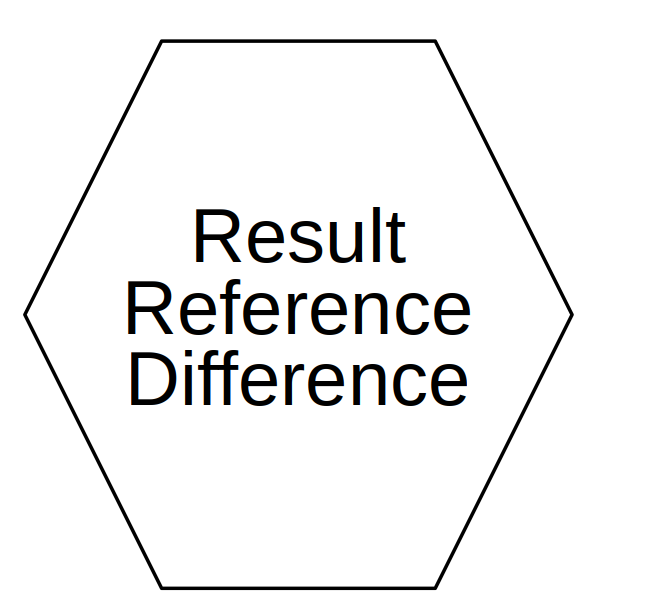
\includegraphics[width=0.15\textwidth]{hex_description}}
\end{frame}

\begin{frame}{IAEA -- No Reflector $\albedo=0.125$}
  \begin{itemize}
    \item Two-dimensional.
    \item Pressurized Water Reactor (PWR).
    \item Two-group.
    \item Originally cartesian but converted to hexagonal in \cite{chao}.
  \end{itemize}
  % nore0125
  \begin{table}
    \begin{center}
      %\caption{IAEA Benchmark Convergence Study. No Reflector. $\albedo = 
      %  0.125$.}
      \label{tab:iaea_nore0125}
      \begin{threeparttable}
        \begin{tabular}{cccc}
          \toprule
          Refine & $\keff$ & $\keff$ error \units{pcm} & $\keff$ ratio \\
          \midrule
          \csvreader[
            late after line=\\,
            late after last line=\\,]
            {../ch03_diffusionResults/data/iaea_nore0125.csv}{}
            {\csvcoli & \csvcolvi & \csvcolvii & \csvcolviii}
          Ref. \tnote{$\dagger$} & 0.991378 \\
          \bottomrule
        \end{tabular}
        \begin{tablenotes}
          \item[$\dagger$] See \cite{chao}.
        \end{tablenotes}
      \end{threeparttable}
    \end{center}
  \end{table}
\end{frame}

\begin{frame}{IAEA -- No Reflector $\albedo=0.500$}
  \begin{itemize}
    \item Two-dimensional.
    \item Pressurized Water Reactor (PWR).
    \item Two-group.
    \item Originally cartesian but converted to hexagonal in \cite{chao}.
  \end{itemize}
  % nore0500
  \begin{table}
    \begin{center}
      %\caption{IAEA Benchmark Convergence Study. No Reflector. $\albedo = 
      %  0.500$.}
      \label{tab:iaea_nore0500}
      \begin{threeparttable}
        \begin{tabular}{cccc}
          \toprule
          Refine & $\keff$ & $\keff$ error \units{pcm} & $\keff$ ratio \\
          \midrule
          \csvreader[
            late after line=\\,
            late after last line=\\,]
            {../ch03_diffusionResults/data/iaea_nore0500.csv}{}
            {\csvcoli & \csvcolvi & \csvcolvii & \csvcolviii}
          Ref. \tnote{$\dagger$} & 0.978077 \\
          \bottomrule
        \end{tabular}
        \begin{tablenotes}
          \item[$\dagger$] See \cite{chao}.
        \end{tablenotes}
      \end{threeparttable}
    \end{center}
  \end{table}
\end{frame}

\begin{frame}{IAEA -- Reflector $\albedo=0.125$}
  \begin{itemize}
    \item Two-dimensional.
    \item Pressurized Water Reactor (PWR).
    \item Two-group.
    \item Originally cartesian but converted to hexagonal in \cite{chao}.
  \end{itemize}
  % refl0125
  \begin{table}
    \begin{center}
      %\caption{IAEA Benchmark Convergence Study. With Reflector. $\albedo = 
      %  0.125$.}
      \label{tab:iaea_refl0125}
      \begin{threeparttable}
        \begin{tabular}{cccc}
          \toprule
          Refine & $\keff$ & $\keff$ error \units{pcm} & $\keff$ ratio \\
          \midrule
          \csvreader[
            late after line=\\,
            late after last line=\\,]
            {../ch03_diffusionResults/data/iaea_refl0125.csv}{}
            {\csvcoli & \csvcolvi & \csvcolvii & \csvcolviii}
          Ref. \tnote{$\dagger$} & 1.006630 \\
          \bottomrule
        \end{tabular}
        \begin{tablenotes}
          \item[$\dagger$] See \cite{chao}.
        \end{tablenotes}
      \end{threeparttable}
    \end{center}
  \end{table}
\end{frame}

\begin{frame}{IAEA -- Reflector $\albedo=0.500$}
  \begin{itemize}
    \item Two-dimensional.
    \item Pressurized Water Reactor (PWR).
    \item Two-group.
    \item Originally cartesian but converted to hexagonal in \cite{chao}.
  \end{itemize}
  % refl0500
  \begin{table}
    \begin{center}
    %\caption{IAEA Benchmark Convergence Study. With Reflector. $\albedo = 
    %  0.500$.}
    \label{tab:iaea_refl0500}
      \begin{threeparttable}
        \begin{tabular}{cccc}
          \toprule
          Refine & $\keff$ & $\keff$ error \units{pcm} & $\keff$ ratio \\
          \midrule
          \csvreader[
            late after line=\\,
            late after last line=\\,]
            {../ch03_diffusionResults/data/iaea_refl0500.csv}{}
            {\csvcoli & \csvcolvi & \csvcolvii & \csvcolviii}
          Ref. \tnote{$\dagger$} & 1.005507 \\
          \bottomrule
        \end{tabular}
        \begin{tablenotes}
          \item[$\dagger$] See \cite{chao}.
        \end{tablenotes}
      \end{threeparttable}
    \end{center}
  \end{table}
\end{frame}

\begin{frame}{Three-Dimensional Problem Analysis}
  Typically more useful to compare control rod worth measurement.
  \begin{itemize}
    \item Case A. Control rods fully removed.
    \item Case B. Control rods partially inserted.
    \item Case C. Control rods fully inserted.
  \end{itemize}
  \begin{align}
    \label{eq:rodworth}
    \text{Rod Worth}_x \units{$\Delta k$} &= \frac{\keffsub{A} - \keffsub{x}}
      {\keffsub{A} \, \keffsub{x}} &\qquad x=\{B,C\} \\
    \label{eq:roddifference}
    \text{Rod Difference}_x \units{$\% \Delta k$} &= (\keffsub{A} - \keffsub{x}) 
      \times 100 \% &\qquad x=\{B,C\} \\
  \end{align}
\end{frame}

\begin{frame}{MONJU}
  \begin{itemize}
    \item Three-dimensional.
    \item Sodium-cooled Fast Reactor (SFR).
    \item Three-group.
    \item Fission spectrum, $\chi$ not provided and instead selected for
      benchmark agreement.
  \end{itemize}
  \begin{table}
    \begin{center}
      %\caption{MONJU Benchmark Rod Worth Results. \cite{monjuBenchmark}}
      \label{tab:monju}
      \begin{threeparttable}
        \begin{tabular}{ccll}
          \toprule
          Pattern & $\keff$ & Rod Worth \units{$\Delta k$} & 
            Rod Difference \units{\%$\Delta k$} \\
          \midrule
          A&1.056816&               &            \\
          B&1.031623&0.023 (2.51E-5) \tnote{$\dagger$} &2.52 (-0.07)\\
          C&1.006519&0.047 (1.77E-3)&5.03 (0.04) \\
          \bottomrule
        \end{tabular}
        \begin{tablenotes}
          \item[$\dagger$] Value in parentheses is difference to reference
            value from \cite{monjuBenchmark}.
        \end{tablenotes}
      \end{threeparttable}
    \end{center}
  \end{table}
\end{frame}

\begin{frame}{KNK}
  \begin{itemize}
    \item Three-dimensional.
    \item Sodium-cooled Fast Reactor (SFR).
    \item Four-group.
    \item Reference data is a transport problem.
  \end{itemize}
  \begin{table}
    \begin{center}
      %\caption{KNK Benchmark Rod Worth Results.}
      \label{tab:knk}
      \begin{threeparttable}
        \begin{tabular}{ccll}
          \toprule
          Pattern & $\keff$ & Rod Worth \units{$\Delta k$} & 
            Rod Difference \units{\%$\Delta k$} \\
          \midrule
          A&1.061752&               &            \\
          B&0.942404&0.119 (1.55E-2) \tnote{$\dagger$} &11.93 (0.75)\\
          C&0.829829&0.263 (3.99E-2)&23.19 (1.67)\\
          \bottomrule
        \end{tabular}
        \begin{tablenotes}
          \item[$\dagger$] Value in parentheses is difference to reference
            value from \cite{takedaBenchmark}.
        \end{tablenotes}
      \end{threeparttable}
    \end{center}
  \end{table}
\end{frame}
